\newpage
\section{Metodologia Experimental}

\subsection{Materiais}
O material utilizado foi:

\begin{itemize}
\item Placa com conversor buck disponível no laboratório.
\item CI 4050.
\item Resistor de 10K $\Omega$.
\item Fonte de alimentação.
\item Osciloscópio.
\item Multímetro.
\item Resistor variável de potência (50 $\Omega$).
\end{itemize}

Para execução do experimento, faz-se necessário executar os seguintes passos:

\begin{enumerate}
\item montar o circuito gerador de onda quadrada conforme a figura \ref{f_gera_onda}, alimentando o CI com 12V;
\item ajustar o gerador de funções para 100KHz, com razão cíclica de 50 \%;
\item conectar os multímetros à placa do conversor buck como mostrado na figura \ref{f_buck};
\item ajustar a tensão de entrada para 30V;
\item variar a carga de modo a incrementar à corrente de saída em 300mA, mantendo a tensão de saída fixa em 15V;
\item anotar o valor da tensão de entrada e saída e da corrente de entrada e saída;
\item repetir os passos 5 e 6 até que a corrente de saída seja 3A ;
\item ajustar a tensão de entrada para 20V e repetir os passos 5,6 e 7;
\item analisar a forma de onda na chave do conversor.
\end{enumerate}

\begin{figure}[H]
	\centering
	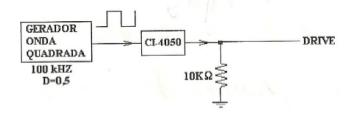
\includegraphics[scale=0.8]{Imagens/gera_onda.jpg}
	\caption{Gerador de onda quadrada.}
	\label{f_gera_onda}
\end{figure}

\begin{figure}[H]
\centering
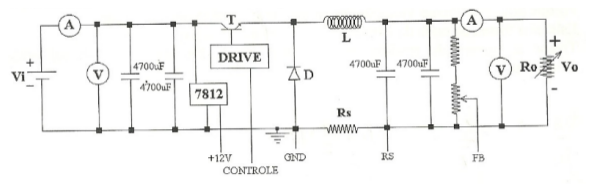
\includegraphics[scale=0.5]{Imagens/buck.jpg}
\caption{Conversor buck.}
\label{f_buck}
\end{figure}
